\chapter{量子统计}\label{ch:b3:quantum-statistics}

铜的导电电子是一种气体，其密度
是空气的一千倍，然而它们对铜的热容几乎毫无贡献——
这一难题困扰经典物理学长达五十年。一团
铷原子云被冷却至千万分之一开尔文，突然坍缩成
一个深达一万个原子的单一量子态。
一颗质量与太阳相当、尺寸与地球相当的死亡恒星
拒绝进一步收缩，仅靠泡利不相容原理支撑。
这三者同属物理学的同一章：
当 $n\lambda_T^3 \sim 1$ 时，气体会发生什么，
而\cref{ch:b3:grand-canonical}中的占据数公式
则会偏离玻尔兹曼分布。费米子构成“海”——冷、刚、受压；玻色子形成凝聚体——
群聚、相干、超流。在费米海沉默的多数与凝聚体的奔涌之间，
是现代凝聚态与低温物理的大部分内容，
同时也决定着
恒星的命运。

\section{占据数气体}

\begin{proposition}[量子气体的基本方法]\label{prop:b3:quantum-statistics:machinery}
\index{态密度}
对于箱中的无相互作用粒子，能级上的求和
化为对态密度的积分，其中态密度见
\cref{prop:b3:schrodinger-three-dimensions:counting}（每个
自旋态，$g(\epsilon) = (V/4\pi^2)(2m/\hbar^2)^{3/2}\sqrt\epsilon$）：
\[
N = \int_0^\infty g(\epsilon)\,\bar n(\epsilon)\,\dd\epsilon ,
\qquad
E = \int_0^\infty g(\epsilon)\,\bar n(\epsilon)\,\epsilon\,
\dd\epsilon ,
\]
其中 $\bar n$ 为费米–狄拉克或玻色–爱因斯坦占据数。第一式确定
$\mu(T, n)$；第二式给出
热力学性质。在稀薄极限 $n\lambda_T^3 \ll 1$ 下，两种统计
都退化为玻尔兹曼分布，经典气体得以恢复；
量子效应则始于波包开始相互重叠之处。
\end{proposition}
\admitted

\section{费米海}

\begin{theorem}[简并费米气体]\label{thm:b3:quantum-statistics:fermi}
\index{费米能}\index{简并压}
在 $T = 0$ 时，费米子填满直到\emph{费米
能}的每一个能级，
\[
E_{\text{F}} = \frac{\hbar^2}{2m}\,(3\pi^2n)^{2/3}
\qquad (\text{自旋 } \tfrac12) ,
\]
每个粒子的平均能量为 $\tfrac35 E_{\text{F}}$，并具有
\emph{简并压}
\[
P = \frac25\,n\,E_{\text{F}} \;\propto\; n^{5/3} :
\]
绝对零度下的压强，纯属量子效应——
它是每种金属电子气体刚性的来源，也是死亡恒星
得以支撑的根源。在 $0 < T \ll T_{\text{F}} = E_{\text{F}}/k_{\text{B}}$ 时，
只有距表面 $\sim k_{\text{B}}T$ 以内的电子，
方能对此\emph{费米海}中的任何扰动作出响应，其占比
约为 $\sim T/T_{\text{F}}$，是理解金属行为的关键。
\end{theorem}

\begin{proof}[部分证明]
将 $g(\epsilon)$ 积分至 $E_{\text{F}}$：由 $N = \int_0^{
E_{\text{F}}}g\,\dd\epsilon$ 反解即得所述的 $E_{\text{F}}$
（见\cref{exo:b3:schrodinger-three-dimensions:8}）；$\langle\epsilon
\rangle = \tfrac35 E_{\text{F}}$（再做一次积分）。压强：
压缩箱体使每个能级按 $V^{-2/3}$ 升高，故 $E
\propto V^{-2/3}$，从而 $P = -\partial E/\partial V = \tfrac23 E/V$
——代入 $E = \tfrac35 NE_{\text{F}}$，即得所述规律。
\end{proof}

\begin{omfigure}
\begin{tikzpicture}
  \begin{axis}[omaxis, axis x line=bottom, axis y line=left,
    width=11.2cm, height=5.2cm, xmin=0, xmax=1.6, ymin=0, ymax=1.2,
    xlabel={$\epsilon/E_{\text{F}}$}, ylabel={占据数 $\bar n$},
    xlabel style={at={(axis description cs:0.5,-0.11)}, anchor=north},
    xtick={1}, ytick={0.5,1}, clip=false]
    \addplot[omDef, very thick, domain=0:1.6, samples=250]
      {1/(exp((x-1)/0.05)+1)};
    \addplot[gray, dashed, domain=0:1] {1};
    \fill[omThm!25] (axis cs:0.85,0) -- (axis cs:0.85,0.953)
      .. controls (axis cs:0.95,0.85) .. (axis cs:1.0,0.5)
      .. controls (axis cs:1.05,0.15) .. (axis cs:1.15,0.047)
      -- (axis cs:1.15,0) -- cycle;
    \node[omThm, font=\scriptsize, anchor=west] at (axis cs:1.07,0.72)
      {热壳层，$\sim k_{\text{B}}T$};
    \draw[->, omThm] (axis cs:1.06,0.66) -- (axis cs:1.0,0.47);
    \node[font=\scriptsize, anchor=west] at (axis cs:0.07,0.35)
      {深能级冻结};
  \end{axis}
\end{tikzpicture}

{\small $T \ll T_{\text{F}}$ 时的费米海：占据数为一个略有弥散的阶跃。
深层电子无法散射、吸收或作出响应；
所有可用态均已被占满，金属物理的全部内容都发生于
表面的薄热壳层之中。}
\end{omfigure}

\begin{example}[热容之谜的解决]\label{ex:b3:quantum-statistics:heat}
\index{电子热容}
经典地看，铜中每个原子的自由电子应给热容贡献 $\tfrac32
k_{\text{B}}$，使热容比杜隆–珀蒂值高出 $50\%$。
实测值在室温下约为 $1\%$。费米海
可以解释此现象：取 $T_{\text{F}} \approx \qty{8e4}{K}$，只有
占比约 $\sim T/T_{\text{F}} \approx 0.4\%$ 的电子可被热激发，
每个电子被激发的能量约为 $\sim k_{\text{B}}T$：
\[
C_{\text{el}} \approx \frac{\pi^2}{2}\,
Nk_{\text{B}}\,\frac{T}{T_{\text{F}}}
\]
（精确的索末菲系数；
见\cref{exo:b3:quantum-statistics:12}）。线性于 $T$ 的这一项
在常温下被晶格的 $T^3$ 项所淹没，
在几开尔文以下则\emph{占主导}——恰如量热计所测得的，
这一结果一举解决了一个谜题：承载电流的电子
为何并不贡献热容。
\end{example}

\begin{example}[靠不相容性支撑的恒星]\label{ex:b3:quantum-statistics:dwarf}
\index{白矮星}
白矮星（见\cref{exo:b3:identical-particles:11}）
以电子简并压强平衡引力。由于 $P \propto
n^{5/3}$ 随恒星收缩而增长得比引力所需更快，故对任意适度的质量都存在平衡半径——
并伴有颇为诡异的标度律
$R \propto M^{-1/3}$：\emph{越重的白矮星
越小}。压缩得更厉害时，电子变为相对论性，
压强律软化为 $n^{4/3}$，平衡在某一唯一质量处被打破，
此即钱德拉塞卡极限 $M_{\text{Ch}} \approx
1.4\,M_\odot$（见\cref{pb:b3:quantum-statistics:1}）——超过此质量，
便坍缩为中子星：一个处于核密度下的中子费米海，
同样的物理，只是密度高出 $10^{14}$ 倍。
\end{example}

\section{玻色狂潮}

\begin{theorem}[玻色–爱因斯坦凝聚]\label{thm:b3:quantum-statistics:bec}
\index{玻色–爱因斯坦凝聚}
对于 $N$ 个守恒玻色子组成的气体，激发态至多能容纳
$N_{\max}(T) = 2.612\,V/\lambda_T^3$ 个粒子（即
$g\bar n_{\text{BE}}$ 在其上限 $\mu \to 0$ 处的积分）。在
临界温度以下，
\[
k_{\text{B}}T_{\text{c}} = \frac{2\pi\hbar^2}{m}
\Big(\frac{n}{2.612}\Big)^{2/3}
\quad\text{ (等价地 } n\lambda_{T_{\text{c}}}^3 = 2.612
\text{)} ,
\]
多余的粒子别无去处，只能进入唯一的基态：一个
\emph{宏观}布居
\[
\frac{N_0}{N} = 1 - \Big(\frac{T}{T_{\text{c}}}\Big)^{3/2}
\]
凝聚到同一个量子态中——物质表现为一个巨大的
波函数。该凝聚由爱因斯坦于 1925 年根据玻色的光子统计预言，
并于 1995 年在稀薄铷气中实现，所处
温度 $T_{\text{c}} \approx \qty{100}{nK}$（2001 年诺贝尔奖），
其标志是特征性的\emph{双峰}速度分布：一团热云，
中心升起一根零速度凝聚态的尖峰。
\end{theorem}
\admitted

\begin{omfigure}
\begin{tikzpicture}
  \begin{axis}[omaxis, axis x line=bottom, axis y line=left,
    width=6.6cm, height=5.0cm, xmin=0, xmax=1.35, ymin=0, ymax=1.1,
    xlabel={$T/T_{\text{c}}$}, ylabel={$N_0/N$},
    xlabel style={at={(axis description cs:0.5,-0.12)}, anchor=north},
    xtick={0.5,1}, ytick={0.5,1}, clip=false]
    \addplot[omDef, very thick, domain=0:1, samples=100]
      {1-x^1.5};
    \addplot[omDef, very thick, domain=1:1.35] {0};
    \node[omDef, font=\scriptsize, anchor=west] at (axis cs:0.1,0.25)
      {凝聚份额};
  \end{axis}
  \begin{axis}[omaxis, axis x line=bottom, axis y line=left,
    width=6.6cm, height=5.0cm, xmin=-3, xmax=3, ymin=0, ymax=1.35,
    xshift=7.2cm,
    xlabel={速度}, ylabel={原子数},
    xlabel style={at={(axis description cs:0.5,-0.12)}, anchor=north},
    xtick=\empty, ytick=\empty, clip=false]
    \addplot[omExo, thick, domain=-3:3, samples=120]
      {0.42*exp(-x*x/1.8)};
    \addplot[omThm, very thick, domain=-3:3, samples=200]
      {0.42*exp(-x*x/1.8)+0.85*exp(-x*x/0.045)};
    \node[omExo, font=\scriptsize, anchor=west] at (axis cs:1.15,0.5)
      {热云};
    \node[omThm, font=\scriptsize, anchor=west] at (axis cs:0.3,1.2)
      {凝聚尖峰};
  \end{axis}
\end{tikzpicture}

{\small 左：$T_{\text{c}}$ 以下，基态的布居
变为宏观量。右：1995 年的特征图像——释放并
成像后，云团呈现宽广的热分布，中心有一个狭窄的
零速度尖峰：一个量子态，照相机即可看到。}
\end{omfigure}

\begin{example}[氦，资深超流体]\label{ex:b3:quantum-statistics:helium}
\index{超流性}
液态 $^4$He（玻色子）在 $T_\lambda = \qty{2.17}{K}$ 时转变为
\emph{超流体}：通过最细的毛细管时黏度为零，
能沿容器壁形成薄膜流动，产生喷泉效应，以及
环量以 $h/m$ 为单位量子化——这是凝聚体的
宏观相位在起作用。与理想气体的预言
（对氦的密度而言为 $\qty{3.1}{K}$）相比，相互作用使其有所偏移，但
显然是同一现象。费米子 $^3$He 不能单独凝聚：
其原子必须先\emph{配对}（如同超导体中的电子，
见\cref{ch:b3:electrons-in-solids}）形成复合玻色子——
超流随之出现，但温度为 \qty{2.6}{mK}，
低了一千倍：两种同位素，一个道理——统计
决定命运。
\end{example}

\begin{method}[何种统计，何种区域]\label{met:b3:quantum-statistics:method}
(1) 先计算 $n\lambda_T^3$：$\ll1$ 表示可用玻尔兹曼统计，
第 17 章即已足够。(2) 简并费米子：用
$E_{\text{F}}$ 与 $T/T_{\text{F}}$ 来思考；响应（热容、
磁化率、散射）都含因子 $T/T_{\text{F}}$，或
只探测费米面。(3) 简并玻色子：比较 $T$
与 $T_{\text{c}}$；低于其时，将气体分为凝聚体与
热云两部分。(4) 压强：费米子刚度 $n^{5/3}$（或
相对论情形的 $n^{4/3}$），与任何压缩因素相抗衡。(5) 复合粒子：
数出组成的费米子数以确定统计性质——
并记住，配对可以使一种统计转化为另一种。
\end{method}

\begin{omfigure}

\includegraphics[width=0.58\linewidth]{images/book5/ai/b5-25-superconductor-levitation.jpg}

{\small 超导体使磁铁的磁场线被排开而悬浮：低于其临界温度时，电子流体凝聚为单一的宏观量子态——简并物理，将磁铁托在空中。}
\end{omfigure}

\section{练习}

\begin{exercise}[$\star$]\label{exo:b3:quantum-statistics:1}
计算以下各情形的 $E_{\text{F}}$ 与 $T_{\text{F}}$：(a) 铜
($n = \qty{8.5e28}{m^{-3}}$)；(b) 钠（$\qty{2.5e28}{m^{-3}}$）；
(c) 液态 $^3$He（$\qty{1.6e28}{m^{-3}}$，$m = 3u$）；(d) 将它们
与室温相比，并说明各自何时处于简并态。
\end{exercise}

\begin{exercise}[$\star$]\label{exo:b3:quantum-statistics:2}
(a) 证明 $\langle\epsilon\rangle = \tfrac35 E_{\text{F}}$ 在 $T =
0$ 时成立。(b) 计算铜中电子的均方根速率。(c) 该
速率经典地对应何种温度？(d) 为什么冷金属中的电子
能以光速的百分之一运动，
却不向外辐射这些能量？
\end{exercise}

\begin{exercise}[$\star$]\label{exo:b3:quantum-statistics:3}
铜中电子的简并压强：(a) 计算 $P =
\tfrac25 nE_{\text{F}}$ 的值，分别以帕斯卡与标准大气压为单位。(b) 金属为何不会爆炸
（是什么在将其拉回）？(c) 该压强抵抗压缩，
请将其与金属的低压缩性相联系。(d) 估算体积模量
$K \sim \tfrac53 P$，并与铜的实测值
\qty{140}{GPa} 比较。
\end{exercise}

\begin{exercise}[$\star$]\label{exo:b3:quantum-statistics:4}
玻色–爱因斯坦凝聚的阈值。(a) 计算铷-87 的 $T_{\text{c}}$（$m =
\qty{1.44e-25}{kg}$），在 $n = \qty{e20}{m^{-3}}$ 时。(b) 在相同的
$n$ 下，氢原子的 $T_{\text{c}}$ 为多少？(c)
为何实验采用纳开尔文量级的稀薄气体，
而不采用毫开尔文量级的稠密气体（高密度、低温下
会发生什么化学变化）？(d) 检验一致性规则 $n\lambda_{T_c}^3
= 2.612$，代入你的铷数据。
\end{exercise}

\begin{exercise}[$\star\star$]\label{exo:b3:quantum-statistics:5}
两种热容。在金属中，$C = \gamma T +
\beta T^3$（电子；晶格）。(a) 利用
\cref{ex:b3:quantum-statistics:heat}，以及类德拜型的晶格
项 $\beta T^3 = 234\,Nk_{\text{B}}(T/\theta_{\text{D}})^3$，
估算铜的交叉温度
（$\theta_{\text{D}} = \qty{343}{K}$，$T_{\text{F}} =
\qty{8.2e4}{K}$）。(b) 在 \qty{300}{K} 时，电子所占的
百分比为多少？(c) 在 \qty{0.1}{K} 时呢？(d) 实验者为何以 $C/T$
对 $T^2$ 作图，这条直线的截距与斜率
分别给出什么？
\end{exercise}

\begin{exercise}[$\star\star$]\label{exo:b3:quantum-statistics:6}
一颗白矮星，质量为一个太阳质量（$M = \qty{2e30}{kg}$），
半径为地球半径（$R = \qty{6.4e6}{m}$），每两个核子含一个电子。(a)
计算 $n_{\text{e}}$ 与 $E_{\text{F}}$（使用非相对论
公式）。(b) 将 $E_{\text{F}}$ 与 $m_{\text{e}}c^2$ 比较，
并与内部温度 \qty{e7}{K} 下的 $k_{\text{B}}T$ 比较，
同时论证“冷”与“近似相对论”两种说法。(c) 将简并压强 $\tfrac25 nE_{\text{F}}$ 与
引力压强估计 $\sim GM^2/R^4$ 比较：是否为同一数量级？
(d) 若 $M$ 增大，天平两侧各自
会发生什么定性变化？
\end{exercise}

\begin{exercise}[$\star\star$]\label{exo:b3:quantum-statistics:7}
中子物质。一颗中子星将 $M = 1.4\,M_\odot$ 压缩至 $R
\approx \qty{11}{km}$ 的范围内。(a) 计算中子数密度，并与核密度
（$\qty{2.3e17}{kg/m^3}$）比较。(b) 计算中子的 $E_{\text{F}}$
（非相对论；$m_{\text{n}}c^2
= \qty{939}{MeV}$），并检验中子的相对论程度。(c) 为何该星的电子
会消失（逆 β 衰变：
$\text{e} + \text{p} \to \text{n} + \nu$——是什么使电子的 $E_{\text{F}}$ 为此付出代价）？
(d) 一茶匙这种物质
的质量是多少？
\end{exercise}

\begin{exercise}[$\star\star$]\label{exo:b3:quantum-statistics:8}
无粒子数约束的玻色子。(a) 光子始终有 $\mu = 0$：为何它们
不能发生
\cref{thm:b3:quantum-statistics:bec}所述的凝聚（冷却时气体
反而会怎样）？(b) 铷原子具有的守恒律，
是光子所缺少的哪一条？(c) 2010 年，人们\emph{确实}制得了
光子的玻色–爱因斯坦凝聚，装置为一个充满染料的谐振腔，其中光子达到热化，粒子数
实际上固定：染料谐振腔恢复了哪一要素？
(d) 晶体中的声子：是否会凝聚，为什么？
\end{exercise}

\begin{exercise}[$\star\star$]\label{exo:b3:quantum-statistics:9}
氦的两种同位素。(a) 计算理想气体模型下的 $T_{\text{c}}$
（液态 $^4$He，$n = \qty{2.2e28}{m^{-3}}$，$m = 4u$），并与
$T_\lambda = \qty{2.17}{K}$ 比较。(b) 为何两者的吻合
只是粗略的（“理想”忽略了液体中的什么）？(c) $^3$He 在几乎相同的
密度下直到毫开尔文量级仍保持正常态：说明其
障碍，以及人们所发现的变通办法的本质。(d) 复合粒子的逻辑检验：一个 $^3$He \emph{对}含偶数个费米子
——是玻色子；$^6$Li 含 $3\text{p} + 3\text{n}
+ 3\text{e} = 9$ 个费米子：对其分类，并列举
恰好利用这一 Li–Li 对比的著名冷原子气体实验。
\end{exercise}

\begin{exercise}[$\star\star\star$]\label{exo:b3:quantum-statistics:10}
严格求解 $T_{\text{c}}$。(a) 写出 $N_{\text{激发}} = \int_0^\infty
g(\epsilon)\dd\epsilon/(\eu^{\beta\epsilon} - 1)$（$\mu = 0$），并
令 $x = \beta\epsilon$，将其化简为 $N_{\text{激发}} =
(V/\lambda_T^3)\cdot\frac{2}{\sqrt\pi}\int_0^\infty\frac{\sqrt
x\,\dd x}{\eu^x - 1}$。(b) 已知 $\int_0^\infty\sqrt x\,\dd x/(
\eu^x - 1) = 2.612\,\sqrt\pi/2$，求出上限并
得到 $T_{\text{c}}$。(c) 推导凝聚分数 $1 -
(T/T_{\text{c}})^{3/2}$。(d) 同一论证为何
在二维箱中\emph{不}产生凝聚（$g(
\epsilon)$ 如何变化，积分的
收敛性会发生什么变化）？
\end{exercise}

\begin{exercise}[$\star\star\star$]\label{exo:b3:quantum-statistics:11}
金属为何能凝聚在一起。将金属建模为：电子数密度为
$n$（每个电子的费米能代价 $\propto n^{2/3}$）的电子，被
中和的离子背景吸引（每个电子的库仑得益
$\sim -e^2n^{1/3}/4\pi\varepsilon_0$）。(a) 写出每个电子的
能量 $\epsilon(n) = An^{2/3} - Bn^{1/3}$，并证明它存在
极小值。(b) 证明平衡时电子间距的量级为
$a_0$——金属的密度并非偶然。(c) 估算
极小值处的结合能量级，以 eV 为单位。(d) 简并压在
这一束缚态中起什么作用（是什么阻止了
库仑坍缩）？
\end{exercise}

\begin{exercise}[$\star\star\star$]\label{exo:b3:quantum-statistics:12}
索末菲的壳层，定量化。(a) 论证：$N$ 个电子中，只有
$\sim g(E_{\text{F}})k_{\text{B}}T$ 个位于活跃壳层，每个
电子多携带约 $\sim k_{\text{B}}T$ 的能量：推出 $C_{\text{el}}
\sim g(E_{\text{F}})k_{\text{B}}^2T$（相差一个常数）。(b) 取
$g(E_{\text{F}}) = 3N/2E_{\text{F}}$，还原出 $C_{\text{el}} \sim
Nk_{\text{B}}T/T_{\text{F}}$（精确系数为 $\pi^2/2$）。
(c) 同样的壳层逻辑给出泡利与温度无关的
自旋磁化率：只有壳层电子能够翻转——但壳层随
$T$ 增大，而每项贡献却按 $1/T$ 减小：证明二者
相互抵消。(d) 陈述简并费米子的一般结论：
\emph{每一}种响应都等于经典响应乘以
$\sim T/T_{\text{F}}$，或其仅限于表面的类似量。
\end{exercise}

\begin{omfigure}
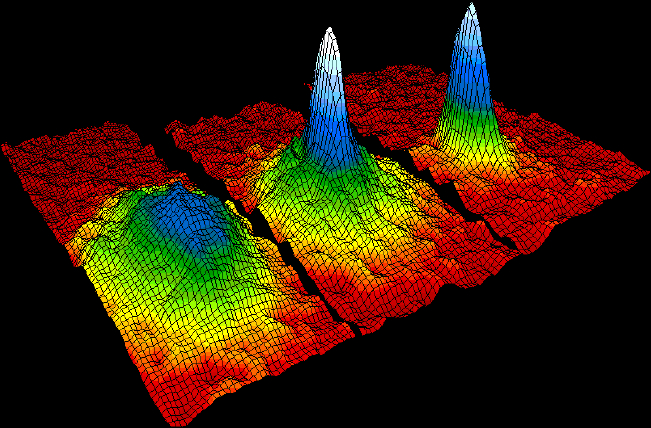
\includegraphics[width=0.55\linewidth]{images/book5/photo-bec-nist.png}

{\small 第一个玻色–爱因斯坦凝聚（NIST/JILA，1995 年，公有领域）：气体自左向右冷却时铷原子的速度分布——热分布的山丘坍缩为凝聚的尖峰，距该预言已过七十年。}
\end{omfigure}

\section{问题：可能的最重白矮星}

\begin{problem}[{周末问题——钱德拉塞卡极限，以及
它所点亮的“标准烛光”}]\label{pb:b3:quantum-statistics:1}
1930 年，年仅十九岁的钱德拉塞卡在前往英国的
船上算出：电子简并只能支撑一颗“死亡”的恒星
达到某一确定质量。这一结果——曾遭爱丁顿
强烈反对——是中子星、黑洞以及揭示宇宙
加速膨胀的超新星“标准烛光”的基础。
本题用标度法将其推导出来。数据：$M_\odot =
\qty{2e30}{kg}$；每 $\mu_e = 2$ 个核子对应一个电子；$m_{\text{
n}} = \qty{1.67e-27}{kg}$；$\hbar c = \qty{3.16e-26}{J.m}$；$G =
\qty{6.67e-11}{N.m^2/kg^2}$。

\medskip\noindent\textbf{第一部分——两种能量的平衡。}
对于质量为 $M$、半径为 $R$ 的恒星，
用标度法处理单位质量的能量。
\begin{enumerate}
  \item 引力势能：$E_{\text{g}} \sim -GM^2/R$——
        回忆其来源。
  \item 电子数 $N_{\text{e}} = M/\mu_e m_{\text{n}}$ 及
        数密度 $n \sim N_{\text{e}}/R^3$：写出非相对论费米能的标度，
        作为 $M$ 和
        $R$ 的函数。
  \item 证明总动能（简并能）的标度为
        $E_{\text{k}} \sim \hbar^2N_{\text{e}}^{5/3}/m_{\text{e}}
        R^2$。
  \item 对 $E_{\text{k}} + E_{\text{g}}$ 关于 $R$ 求极小，并证明
        平衡半径为
        $R \sim \hbar^2 N_{\text{e}}^{-1/3}/(G\,m_{\text{e}}\,
        m_{\text{n}}^2\mu_e^2)$。
  \item 由标度关系 $R \propto M^{-1/3}$ 可知：质量越大的白矮星
        \emph{更小}。这为何已经
        预示着麻烦？
  \item 求 $R$ 在 $M = 1\,M_\odot$ 时的值，并与天狼星 B 的
        实测值 $\approx\qty{5800}{km}$ 比较。
\end{enumerate}

\medskip\noindent\textbf{第二部分——相对论抽走了
地板。}
\begin{enumerate}[resume]
  \item 随 $R$ 减小，$E_{\text{F}}$ 增大：估算
        使 $E_{\text{F}} \sim m_{\text{e}}c^2$ 成立的密度，以及
        对应的白矮星质量区间。
  \item 在超相对论区，每个电子的能量为
        $\sim\hbar c\,n^{1/3}$，证明动能变为
        $E_{\text{k}} \sim \hbar c\,N_{\text{e}}^{4/3}/R$。
  \item 此时两种能量均按 $1/R$ 标度变化，由此得出：
        平衡不再决定半径——应转而比较两者的
        系数。
  \item 令 $\hbar c\,N_{\text{e}}^{4/3} \sim
        GM^2 = G(\mu_em_{\text{n}}N_{\text{e}})^2$，推导
        临界电子数与质量，得到
        \[
        M_{\text{Ch}} \sim
        \Big(\frac{\hbar c}{G\,m_{\text{n}}^2}\Big)^{3/2}
        \frac{m_{\text{n}}}{\mu_e^2} .
        \]
  \item 计算无量纲比值 $\hbar c/Gm_{\text{n}}^2$
        ——物理学中最重要的纯数之一——再求
        以太阳质量为单位的 $M_{\text{Ch}}$（精确处理给出
        $1.4\,M_\odot$）。
  \item 解释该公式：哪三个常数共同起作用，以及
        为何一个\emph{量子}极限施加于\emph{恒星}上，
        仍会含有 $\hbar$？
\end{enumerate}

\medskip\noindent\textbf{第三部分——越过极限之后。}
\begin{enumerate}[resume]
  \item 白矮星因伴星吸积而超过 $M_{\text{Ch}}$ 后，
        接下来由什么支撑它，以及其半径的标度为何
        （在第一部分的半径中，将 $m_{\text{e}}$ 换为 $m_{\text{n}}$，
        并将 $\mu_e$ 换为 1）？
  \item 证明中子星自身的相对论极限与
        $M_{\text{Ch}}$ 处于同一量级——自然只给出
        两倍的宽限（观测最大质量 $\approx
        2.2\,M_\odot$）。超出之后又会如何？
  \item 在坍缩为中子星的过程中，释放的引力能 $\sim GM^2/R_{
        \text{ns}}$ 的引力能被释放：求其在
        $M = 1.4\,M_\odot$、$R = \qty{11}{km}$ 时的值，并与
        太阳整个 \qty{10}{Gyr} 的输出相比较
        （$\sim\qty{1.2e44}{J}$）。
  \item 几乎全部能量在数秒内以中微子形式逸出：哪一次
        1987 年的观测极为精彩地证实了这一图景？
  \item 坍缩核心的反弹与中微子的推动将
        包层抛离，这便是核心坍缩型超新星。请各用一句话，
        将其与\emph{热核}（Ia 型）超新星区分开：后者是白矮星
        在钱德拉塞卡
        阈值处被点燃的超新星。
  \item 为何\emph{在统一的质量}处发生爆轰，会使
        Ia 型超新星几乎完全相同——从而
        可用作“标准烛光”？
\end{enumerate}

\medskip\noindent\textbf{第四部分——烛光与
宇宙。}
\begin{enumerate}[resume]
  \item 标准烛光的视亮度给出其
        距离：陈述平方反比律的逻辑，并说明为什么
        关键词是\emph{标准}。
  \item 1998 年两个团队发现遥远的 Ia 型超新星
        比预期\emph{更暗}：陈述由此得出的推断
        （膨胀在加速——暗能量），并说明
        烛光的可靠性为何是关键。
  \item 用一行列出本题的推理链：泡利 $\to$
        简并压 $\to$ $M_{\text{Ch}}$ $\to$ 均匀
        爆炸 $\to$ 宇宙加速。
  \item 爱丁顿嘲笑这一结果（“一颗恒星在犯
        荒谬的错误”）；钱德拉塞卡获得诺贝尔奖，
        五十三年后：这段经历说明
        在方程推导超出舒适结论时应如何对待它？
  \item 天狼星 B 在 1915 年的光谱暗示其密度为每立方厘米一吨，
        被视为“荒谬”，直到 1926 年费米统计提出后数月，福勒
        便将其解释为简并气体：说明为何
        同一谜题一年前无解，
        一年后却成为常规。
  \item 对数千颗白矮星的巡天发现其质量
        聚集在 $0.6\,M_\odot$ 附近，没有一颗超过
        $\approx1.4\,M_\odot$：这一单一直方图
        证实了本题的哪两个预测？
  \item 概括该命名结果：$(\hbar c/Gm_{\text{n}}^2)^{
        3/2}m_{\text{n}} \approx 1.4\,M_\odot$——三个
        自然常数决定了最重白矮星的上限，也决定
        宇宙中经标定的爆炸的触发质量。
\end{enumerate}
\end{problem}
